% !TeX encoding=utf8
% !TeX spellcheck = de_CH_frami

\chapter{Sensordaten auswerten und aufbereiten}\label{chap:AnalyseReporting}
Im vorangehenden Kapitel wurde beschrieben, wie die Daten mit Hilfe eines Raspberry Pi und F\# gesammelt wurden. Die Aufbereitung, Auswertung und Visualisierung dieser Daten wird in diesem Kapitel beschrieben.


\section{Verwendete Software}
\label{sec:display:software}
Die Daten werden mittels F\# auf einem Linux Mint (ein Ubuntu Ableger) dargestellt. Dazu muss Mono installiert werden. 

Danach werden die Daten mit F\# Data\footcite{FShaprp_Data_2016-06-17} ausgelesen, mit F\# aufbereitet und mit FSharp.Charting\footcite{FSharp_Charting_2016-06-17} dargestellt.

\todo{Evtl. Abschnitt über Visualisierung mit Raspberry PI, wenn noch Zeit}

\subsection{Mono}
Was Mono ist und wie es installiert wird, wurde im \cref{sec:collect:fsharp:variant1:mono} \nameref{sec:collect:fsharp:variant1:mono} beschrieben.

.NET Core wird für F\# Data und FSharp.Charting nicht benötigt. Dadurch entfällt auch die Installation der entsprechenden Komponenten.

\subsection{F\# Data}
\label{sec:display:software:fsharpdata}
F\# Data ist eine Library für den Zugriff auf Daten. Unterstützt werden folgende Formate:
\begin{itemize}
\item CSV
\item HTML
\item JSON
\item XML
\end{itemize}

In dieser Arbeit wurde als Datenformat CSV gewählt, weshalb die nachfolgenden Erklärungen für dieses Format ausgelegt wurde.
Zuerst muss ein Type erstellt werden, welcher für die Zugriff auf die Daten verwendet wird.
\begin{lstlisting}
type Weather = CsvProvider<"http://www.some-weather-service.org/data.csv", ";">
\end{lstlisting}

Dies lädt eine CSV-Datei von der angegebenen Adresse. Es wird erwartet, dass die Erste Zeile die Namen der Spalten enthält. Zum Beispiel:

\begin{lstlisting}
City;Temperature;Rain
London;6 degree celius;25mm/3h
New York;25 degree celius;<1mm/3h
[...]
\end{lstlisting}

Der Zweite Parameter im obigen Code ist ein Semicolon und definiert, welches Zeichen als Trenner der Spalten verwendet wird.

Danach können die Daten geladen werden:
\begin{lstlisting}
let weatherData = SensorData.Load("http://www.some-weather-service.org/data.csv")
\end{lstlisting}

Die Variable weatherData enthält eine Sequenz von dem zuvor erstellten Typen, über welche nun zugegriffen werden kann.

\begin{lstlisting}
let londonWeather = weatherData.Rows |> Seq.Head
let londonTemperature = londonWeather.Temperature
\end{lstlisting}

\subsection{FSharp.Charting}
FSharp.Charting ist eine Library zur Visualisierung von Daten. 
Es werden verschiedene Charts unterstützt:



\begin{figure}[htb]
	\begin{subfigure}[b]{.30\linewidth}
		\centering
		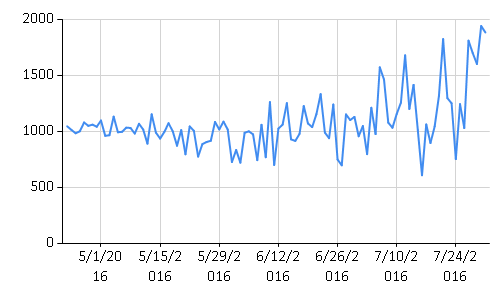
\includegraphics[width=1\linewidth]{images/charting-line.png}
		\caption{Line}
	\end{subfigure}
	\begin{subfigure}[b]{.30\linewidth}
		\centering
		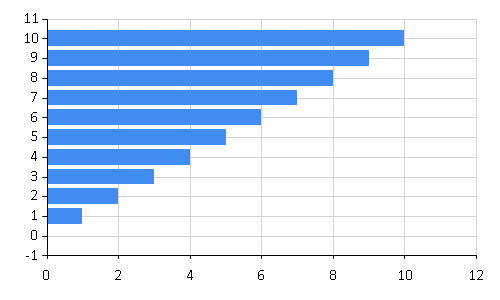
\includegraphics[width=1\linewidth]{images/charting-bar.png}
		\caption{Bar}
	\end{subfigure}
	\begin{subfigure}[b]{.30\linewidth}
		\centering
		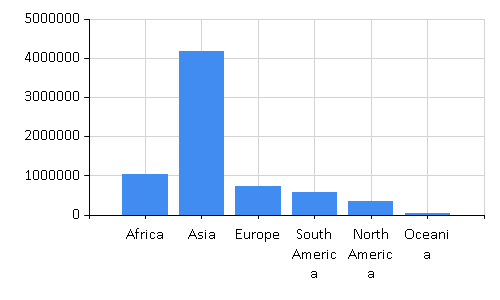
\includegraphics[width=1\linewidth]{images/charting-column.png}
		\caption{Column}
	\end{subfigure}

	\begin{subfigure}[b]{.30\linewidth}
		\centering
		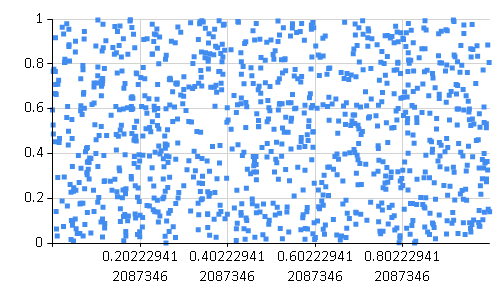
\includegraphics[width=1\linewidth]{images/charting-point.png}
		\caption{Point}
	\end{subfigure}
	\begin{subfigure}[b]{.30\linewidth}
		\centering
		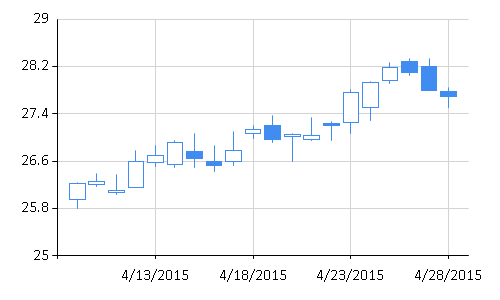
\includegraphics[width=1\linewidth]{images/charting-candlestick.png}
		\caption{Candlestick}
	\end{subfigure}
	\begin{subfigure}[b]{.30\linewidth}
		\centering
		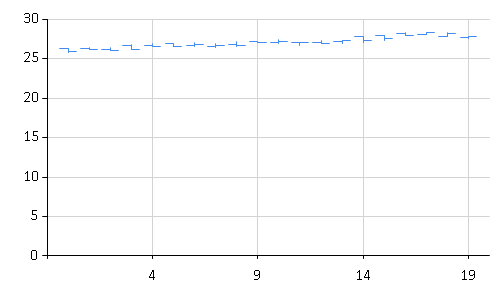
\includegraphics[width=1\linewidth]{images/charting-stock.png}
		\caption{Stock}
	\end{subfigure}

	\begin{subfigure}[b]{.30\linewidth}
		\centering
		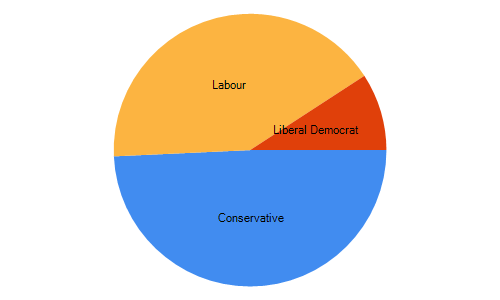
\includegraphics[width=1\linewidth]{images/charting-pie.png}
		\caption{Pie}
	\end{subfigure}
	\begin{subfigure}[b]{.30\linewidth}
		\centering
		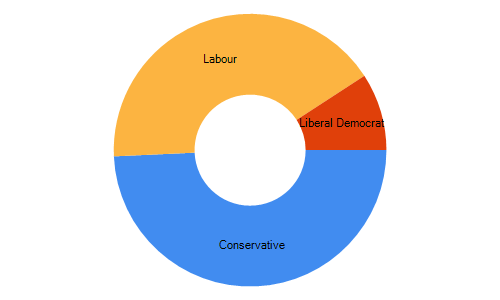
\includegraphics[width=1\linewidth]{images/charting-doughnut.png}
		\caption{Doughnut}
	\end{subfigure}
	\begin{subfigure}[b]{.30\linewidth}
		\centering
		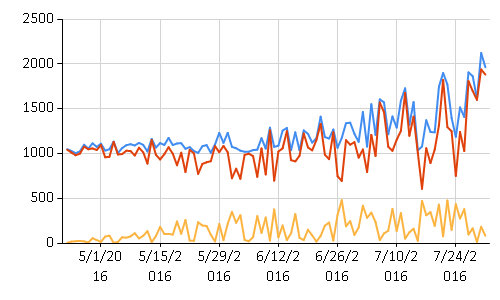
\includegraphics[width=1\linewidth]{images/charting-combine.png}
		\caption{Combine}
	\end{subfigure}
  \caption{Chart Typen von FSharp.Charting}
\end{figure}

Um ein Chart darzustellen, müssen zuerst die benötigen Libraries geladen werden:
\begin{lstlisting}
#I "packages/FSharp.Charting"
#load "FSharp.Charting.fsx"

open FSharp.Charting
open System
\end{lstlisting}

Danach muss eine Sequenz mit Daten befüllt werden:
\begin{lstlisting}
let timesTwo = for x in 1.0 .. 100.0 -> (x, x ** 2.0)
\end{lstlisting}

Schlussendlich kann das Chart dargestellt werden:
\begin{lstlisting}
Chart.Line timesTwo
\end{lstlisting}

Die Ausgabe dieses Codes ist die folgende:
\begin{figure}[H]
  \centering
  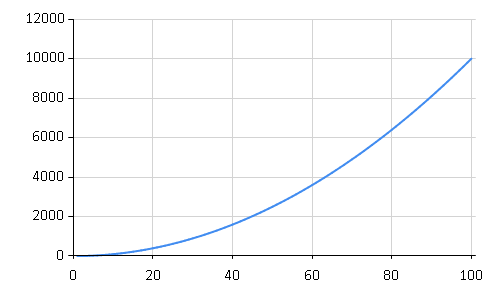
\includegraphics[width=0.6\textwidth]{./images/charting-timestwo.png}
  \caption{Beispiel Chart}
\end{figure}


\section{Dokumentation der Implementation}
Im \cref{sec:display:software} \nameref{sec:display:software} wurde die Software für die Implementation vorgestellt. In diesem Abschnitt wird auf die Umsetzung für dieses Projekt eingegangen. Zuerst wird das Auslesen der Daten, danach die Aufbereitung und zuletzt die Visualisierung erläutert.

\subsection{Auslesen}
\label{sec:display:documentation:reading}
Das Auslesen der Daten mit F\# Data funktionierte wie im \cref{sec:display:software:fsharpdata} \nameref{sec:display:software:fsharpdata} beschrieben. Die Library konnte über den NuGet Package Manager\footcite{NuGet_2016-06-18} geladen und installiert werden.
\begin{lstlisting}
> Install-Package FSharp.Data -Version 2.3.0
\end{lstlisting}

Danach wurde der Typ erstellt und die Daten geladen:
\begin{lstlisting}
type SensorData = CsvProvider<"SensorData-L.csv", ";">
let light = SensorData.Load("SensorData-L.csv")
\end{lstlisting}

Das Skript wurde "`Program.fsx"' genannt und lag im gleichen Ordner wie das File "`Sensor-Datan-L.csv"'. Diese Datei enthält die Daten der Lichtmessung und hatte dieselbe Struktur wie im \cref{sec:AnalyseCollection:application} \nameref{sec:AnalyseCollection:application} beschrieben.

\subsection{Aufbereitung}
\label{sec:display:documentation:manipulation}
Während der Aufbereitung der Daten wurden zwei Methoden definiert:
\begin{lstlisting}
let chunk size list =
    let chunkedValues = list |> Seq.chunkBySize size
    chunkedValues |> Seq.map (fun r -> r |> Seq.averageBy (fun e -> e |> float))

let format (sensorData:SensorData) =
    let values = sensorData.Rows |> Seq.map (fun r -> r.SensorData)
    chunk 1000 values
\end{lstlisting}

\textit{format} nimmt SensorData entgegen und erstellt eine Sequenz mit den Daten der Sensoren. Die CSV-Datei, mit welcher getestet wurde, hat über 100'000 Einträge. Deshalb wurden die Einträge mit der Funktion \textit{chunk} gebündelt.

\textit{chunk} nimmt eine Anzahl und eine Sequenz entgegen. Der erste Parameter gibt an, wie viele Elemente des der Liste zusammengefasst werden sollen. Um im Chart eine begradigte Linie zu erhalten, wird von den zusammengefassten Einträgen noch der Durchschnitt errechnet.

\subsection{Darstellung}
Mit FSharp.Charting wurde nun die zuvor aufbereiteten Daten dargestellt.
Das Verwendung dieser Library gestaltete sich jedoch komplizierter als angenommen.

Zuerst wurde die Library über NuGet installiert:
\begin{lstlisting}
> Install-Package FSharp.Charting 
\end{lstlisting}

Diese funktioniert jedoch nur auf Windows.
Deshalb musste sie deinstalliert und statt dessen "`FSharp.Charting.Gtk"' verwendet werden.

Nun wurde versucht die Daten mit dem Code für das Auslesen und die Aufbereitung (siehe \cref{sec:display:documentation:reading} \nameref{sec:display:documentation:reading} und \cref{sec:display:documentation:manipulation} \nameref{sec:display:documentation:manipulation}) darzustellen:
\begin{lstlisting}
let lightValues = format light
let chart = Chart.Line lightValues
\end{lstlisting}

Mit dem folgenden Befehl wurde versucht, das Chart darzustellen:
\begin{lstlisting}
> fsharpi Program.fsx
\end{lstlisting}

Es erschien jedoch folgende Fehlermeldung:
\begin{lstlisting}
[mono-rt] =================================================================
[mono-rt] Got a SIGSEGV while executing native code. This usually indicates
[mono-rt] a fatal error in the mono runtime or one of the native libraries 
[mono-rt] used by your application.
[mono-rt] =================================================================
\end{lstlisting}

Es gab verschiedene Probleme:
\begin{enumerate}
\item Falsche Imports
\item Darstellung des Charts
\item 'X' Berechtigung
\item Asynchrone Ausführung
\end{enumerate}

\textbf{1. Falsche Imports} \\
Es stellte sich heraus, dass das einfache Einbinden von "`FSharp.Charting.Gtk.fsx"' nicht genügte.
Mit Backtracking der Fehlermeldungen zeigte sich, dass mehrere zusätzliche DLL's benötigt wurden:
\begin{lstlisting}
#I "/usr/lib/cli/gtk-sharp-2.0/"
#I "/usr/lib/cli/gdk-sharp-2.0/"
#I "/usr/lib/cli/atk-sharp-2.0/"
#I "/usr/lib/cli/glib-sharp-2.0/"
#I "bin/Debug/"

#r "gtk-sharp.dll"
#r "gdk-sharp.dll"
#r "atk-sharp.dll"
#r "glib-sharp.dll"
#r "FSharp.Charting.Gtk.dll"
#r "FSharp.Data.DesignTime.dll"
\end{lstlisting}

\textbf{2. Darstellung des Charts} \\
Gemäss Dokumentation reicht für die Darstellung des Charts folgender Code:
\begin{lstlisting}
Chart.Line lightValues
\end{lstlisting}
Dies ist jedoch nur der Fall, wenn über F\# Interactive die einzelnen Befehle einzeln ausgeführt werden. Dies führt einen Handler aus welcher das Chart anzeigt\footcite{FSharp_Charting_Point_and_Line_Charts_2016-06-18}. Als fsx Programm muss zusätzlich noch die Methode "`ShowChart"' ausgeführt werden.

\begin{lstlisting}
Chart.Line(lightValues).ShowChart()
\end{lstlisting}

\textbf{3. X Berechtigung} \\
Das Programm hat keine Berechtigung, um ein neues Fenster zu öffnen. Deshalb muss mit dem Befehl "`xhost +localhost"' dem localhost (der eigenen Computer) erlaubt werden, ein Fenster zu öffnen.

\textbf{4. Asynchrone Ausführung} \\
Mit dem Code bis an hin konnte ein Fenster geöffnet werden, und es wurde auch ein Chart angezeigt. Dieses konnte jedoch nicht mehr geschlossen werden, weil der Thread, auf welchem das Programm läuft, vom Chart besetzt war. Deshalb musste das Skript so umgebaut werden, dass die Ausführung asynchron erfolgt.

\textbf{Das Resultat} \\
\begin{lstlisting}
#I "/usr/lib/cli/gtk-sharp-2.0/"
#I "/usr/lib/cli/gdk-sharp-2.0/"
#I "/usr/lib/cli/atk-sharp-2.0/"
#I "/usr/lib/cli/glib-sharp-2.0/"
#I "bin/Debug/"
#I "../packages/Rx-Linq.2.2.5/lib/net40/"

#r "gtk-sharp.dll"
#r "gdk-sharp.dll"
#r "atk-sharp.dll"
#r "glib-sharp.dll"
#r "FSharp.Charting.Gtk.dll"
#r "FSharp.Data.DesignTime.dll"
#r "FSharp.Data.dll"
#r "FSharp.Control.Reactive.dll"
#r "System.Reactive.Linq.dll"

#load "../packages/FSharp.Charting.Gtk.0.90.14/FSharp.Charting.Gtk.fsx"

open FSharp.Charting
open System
open System.Threading
open FSharp.Data

type SensorData = CsvProvider<"SensorData-L.csv", ";">

let chunk size list =
    let chunkedValues = list |> Seq.chunkBySize size
    chunkedValues |> Seq.map (fun r -> r |> Seq.averageBy (fun e -> e |> float))

let format (sensorData:SensorData) =
    let values = sensorData.Rows |> Seq.map (fun r -\section{Verwendete Hardware}> r.SensorData)
    chunk 1000 values

let runApp = async{
    let light = SensorData.Load("SensorData-L.csv")
    let lightValues = format light
    let chart = Chart.Line(lightValues).ShowChart()
    Gtk.Application.Run()
    ignore 0
    }

let runMain  = async{

    printfn "Starting application"
    let! app = Async.StartChild runApp

    printfn "Press any key to exit..."
    let n = Console.ReadKey()
    Gtk.Application.Quit()
    printfn "Bye..."
    }

// run the whole workflow
Async.RunSynchronously runMain  

//1. xhost +localhost
//2. fsharpi Program.fsx
\end{lstlisting}

\section{Resultat}
Schlussendlich konnte mit F\# Code die vom den GrovePi Sensoren erfassten Daten ausgewertet werden. Das Resultat ist zum Beispiel folgendes Diagramm:

\begin{figure}[H]
  \centering
  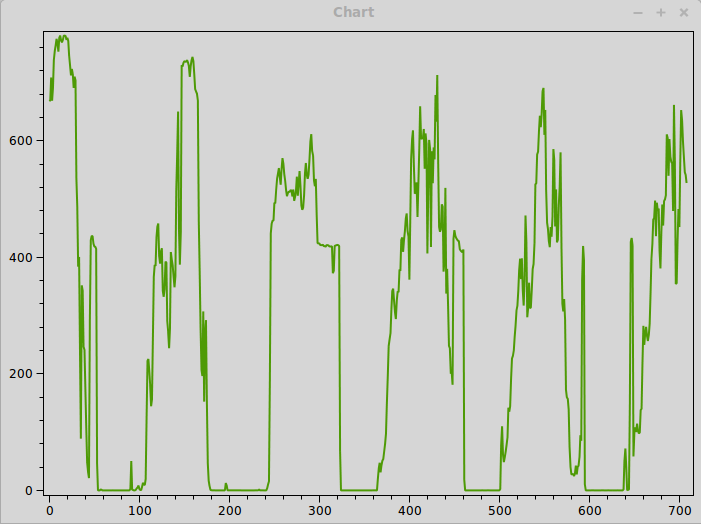
\includegraphics[width=0.6\textwidth]{./images/resultat.png}
  \caption{Resultat: Lichtsensor}
\end{figure}

Das Chart zeigt die Auswertung eines Lichtsensores, welcher vom 27.05.2016 um 13:16 bis am 01.06.2016 um 17:37 Uhr lief (447'639 Sekunden). Gesammelt wurden 708'204 Messungen. Dies macht pro Sekunde 1.58 Messpunkte. Die Darstellung des Chart-Fensters dauerte 4.92 und die Vearbeitung aller Datensätze 5.88 Sekunden.

\todo{Evtl. Vergleich mit Raspberry Pi, wenn noch Zeit}